

\newpage
\chapter{Specifity of the data analysis off a moving proton}
\label{sec:data_an_on_mov_p}
\mbox{}\vspace{-\baselineskip}

During the deuteron target data analysis one encounters specific issues that are completely external to the free proton data analysis. Those of them that originate solely from the fact of initial proton motion are sketched below.  


%\begin{itemize}
\section{Fermi smearing of the invariant mass of the initial particles}
% and its unfolding in the extracted observables
%the need to unfold this smearing in the extracted observable}

For the process of double-pion electroproduction off the proton (as for any other exclusive process) the reaction invariant mass can in general be determined in two ways, i.e. either from the initial particle  four-momenta\footnote[1]{Although the scattered electron is treated as a final particle, here it is classified as ``initial", since it defines the virtual photon, which in turn is attributed to the initial state.} ($W_{i}$) or from the final particle  four-momenta ($W_{f}$) as Eqs.~\eqref{W_fin_1} and~\eqref{W_fin_2} demonstrate\footnote[2]{In electron scattering experiments $W_{i}$ is distorted by the radiative effects, which electrons undergo. The detector resolution also contributes to the difference between experimental values of $W_{i}$ and $W_{f}$.}. 


%\begin{equation}
\begin{eqnarray}
W_{i}&= & \sqrt{(P_{p}+P_{\gamma_{v}})^{2}} \label{W_fin_1} \\
W_{f}&= & \sqrt{(P_{\pi^{+}}+P_{\pi^{-}}+P_{p'})^{2}} \label{W_fin_2}
\end{eqnarray}
%\end{equation}

Here $P_{\pi^{+}}$, $P_{\pi^{-}}$, and $P_{p'}$ are the four-momenta of the final state hadrons, $P_{p}$ is the four-momentum of the initial proton and $P_{\gamma_{v}}=P_{e}-P_{e'}$ the four-momentum of the virtual photon with $P_{e}$ and $P_{e'}$ the four-momenta of the incoming and scattered electrons, respectively. 


%In reactions both on free or moving protons these two values of $W$ are  different due to the fact that $W_{i}$ is distorted by the radiative effects, which electrons undergo, whereas $W_{f}$ is not. In addition to that the detector resolution also contributes to the difference. It also needs to be mentioned that (in contrast to $W_{i }$) $W_{f}$ is affected by the final state interactions (this effect is of minor significance for the free proton experiment). 

To determine $W_{f}$, all final hadrons should be registered, while for the calculation of $W_{i}$ it is sufficient to register the scattered electron. 
In the analyses of exclusive reactions, the latter opportunity allows  to use event samples with one unregistered final hadron, whose four-momentum is reconstructed via the missing mass technique. This approach allows to increase the analyzed statistics (sometimes significantly).


The situation complicates for reactions that happen off the proton that moves as in the deuteron. The motion of the target proton is concealed from the observer and usually is not measured. If all particles in the final state are registered, one can restore the information about the momentum of the target proton via the energy-momentum conservation\footnote[3]{In general the target proton momentum can also be reconstructed by measuring the spectator nucleon.}, however if one of the final hadrons is not registered this information turned out to be totally lost. Therefore the value of $W_{i}$ given by Eq.~\eqref{W_fin_1} turns out to be ill-defined, since $P_{p}$ is not known. This brings us to the choice to either demand the registration of all final hadrons to determine $W_{f}$, which reduces the flexibility of the analysis, or to work under a so-called ``target-at-rest assumption", which assumes the initial proton to be at rest. In the last approach the value of $W_{i}$ appears to be smeared.

As a consequence of this smearing, all extracted observables, which depend on the value of $W$, turned out to be convoluted with a function that is determined by the Fermi motion of the initial proton~\cite{Skorodumina:2015rea}. To retrieve the non-smeared observables, a correction that unfolds this effect should be applied. In order to develop this correction, one needs to simulate properly the investigated exclusive process off the moving proton. 

The simulation of $W$-smearing in TWOPEG-D is described in Sect.~\ref{sect:proc}.

\section{Exclusivity cut in the presence of Fermi smearing}

In order to pick out the exclusive reaction, it is a common practice to perform a so-called ``exclusivity cut" as a final step of the event selection. This is a cut on the missing mass, which is calculated via the energy-momentum conservation from the four-momenta of registered particles and reflects the mass spectrum of the unregistered part. For example, for the reaction $ep\rightarrow e'p'\pi^{+}X$, where the scattered electron and final $p$ and $\pi^{+}$ are registered, the missing mass squared of the unregistered part $X$ is determined in the following way,


 \begin{equation}
 M_{X[\pi^{-}]}^{2}=[P_{e} + P_{p}- P_{e'}- P_{p'}-  P_{\pi^{+}}]^{2}.\label{eq:main_top_mm_nosq}
\end{equation}

The investigation of the distribution of the quantity $M_{X[\pi^{-}]}^{2}$ allows to judge the admixture of any types of background as well as the reliability of the entire event selection. A properly chosen position of the exclusivity cut allows at least to suppress the background contribution or even eliminate it completely and to get rid of the non-physical events.


The missing mass is generally subject to the smearing due to the detector resolution. However, if the target proton moves as in the deuteron, the missing mass is also subject to Fermi smearing due to the inevitability to work under the target-at-rest assumption that originates from the incomplete knowledge about the target motion as well as the final hadron state.

If the data analysis includes the estimation of the detector efficiency (for example with the goal to extract a cross section), then the exclusivity cut should also be applied to the reconstructed Monte-Carlo events. In order to calculate the efficiency correctly, the Monte-Carlo distributions should match the experimental ones as well as possible. Fermi smearing of the experimental distributions demands that the simulation should reproduce it. Therefore, the effects of the Fermi motion should be properly included into the Monte-Carlo simulation\footnote[4]{In addition to Fermi smearing, the experimental missing mass distributions are subject to distortions due to FSI effects~\cite{Skorodumina:2015rea}, which can hardly be simulated. This fact increases the importance of the reliable simulation of Fermi smearing for the proper dealing with the FSI contributions during the data analysis. }. 


Section~\ref{sect:proc} describes the method that is used in TWOPEG-D for the simulation of the particle four-momenta and gives examples of smeared missing mass distributions.


%For reliable channel identification distributions of reconstructed Monte-Carlo events must match experimental ones as well as possible. Fermi smearing of the experimental distributions demands the simulated distributions to reproduce this smearing. Therefore, the effects of Fermi motion must be properly included in the Monte-Carlo simulation.


\section{Transformation to the CMS in the case of moving protons}

For universality purposes the observables are usually extracted in the center-of-mass system (CMS). This implies the transformation of the four-momenta of all particles from the laboratory system (Lab) to the CMS and the subsequent calculation of all kinematical variables from these transformed four-momenta. The description of the kinematical variables for the reaction of double-pion electroproduction off the free proton is given in~\cite{twopeg, Byckling:1971vca,  Fed_an_note:2017}. 



The CMS system is uniquely defined as the system, where the initial proton and the photon move towards each other with the $Z_{CMS}$-axis pointing along the photon direction and the net momentum equal to zero. However, the procedure of the Lab to CMS transformation differs depending on the specifity of the reaction's initial state. 

\begin{figure}[!ht]
\begin{center}
\framebox{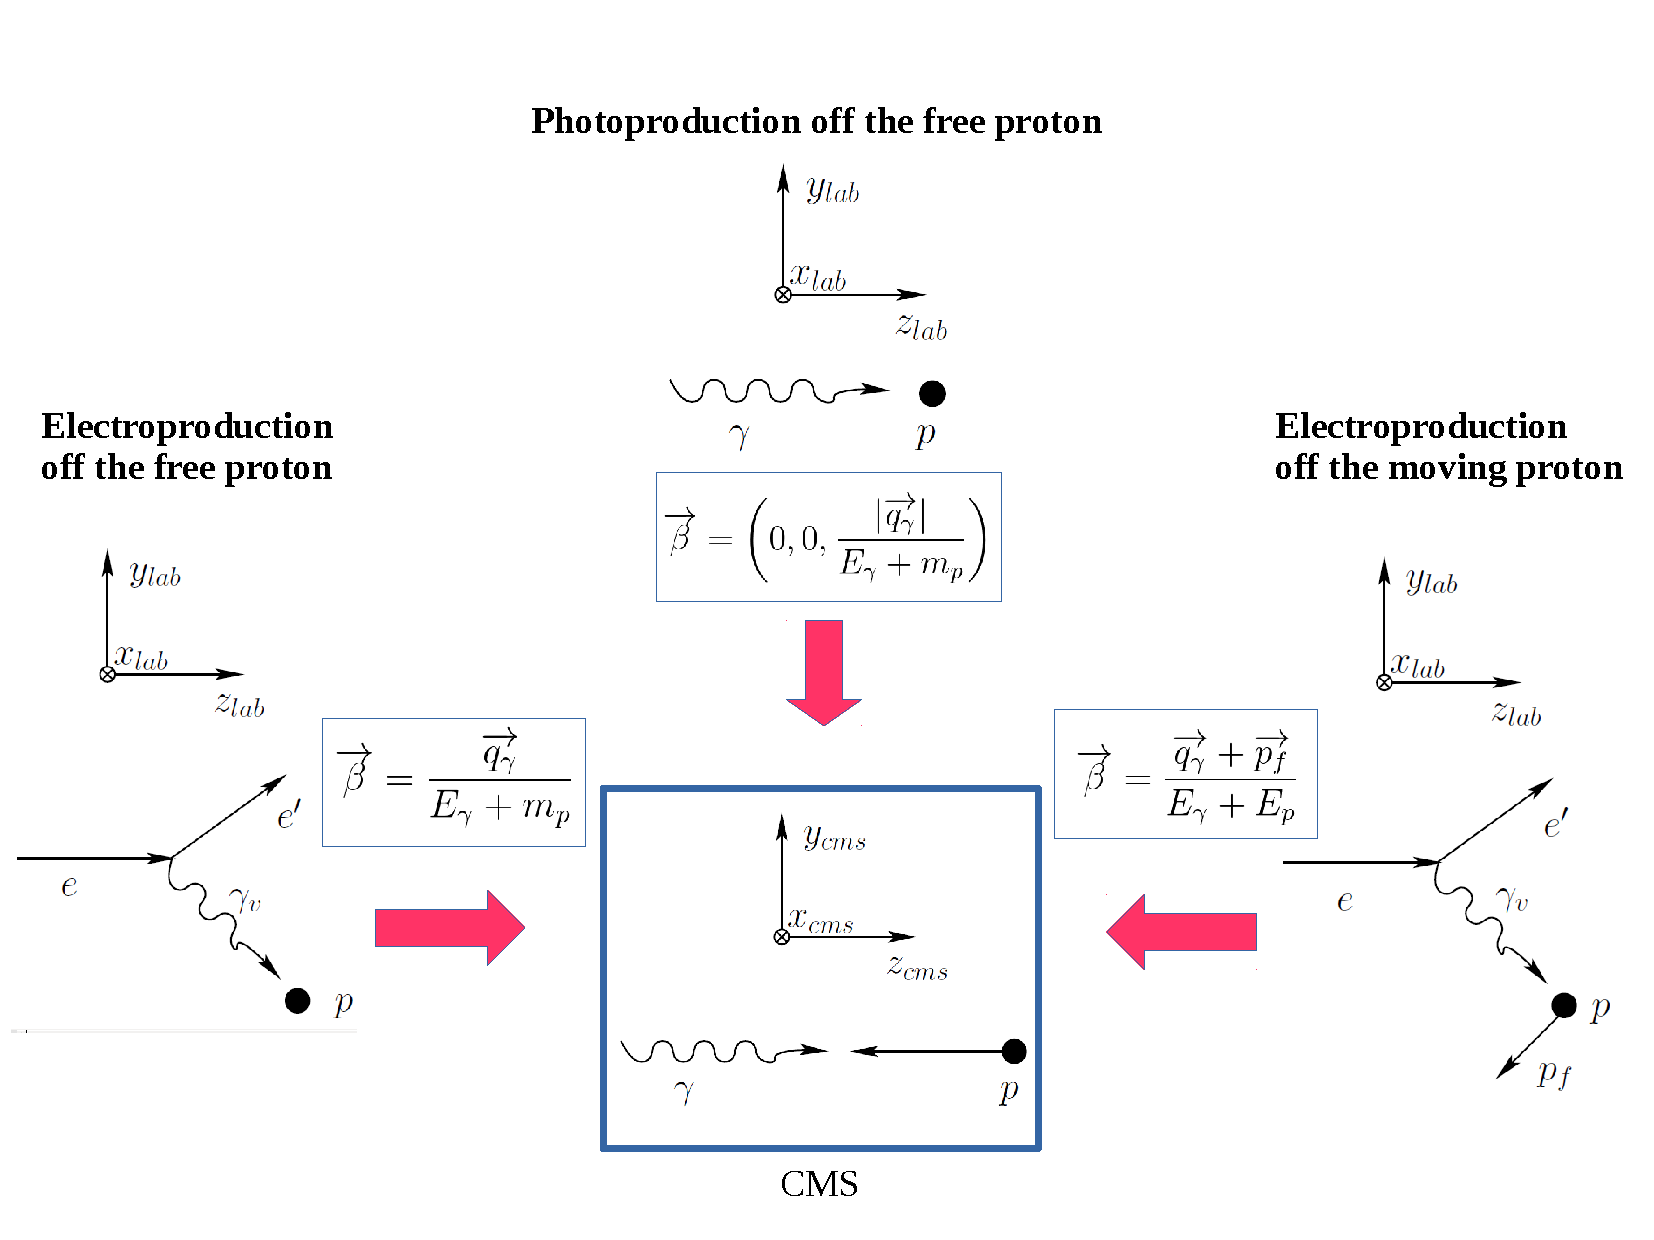
\includegraphics[width=14cm]{pictures/lab_cms_trans3.pdf}}
\end{center}
\caption{\small  The illustration of three options for the experimental specification of the initial state.}
\label{fig:lab_to_CMS}
\end{figure}

Figure~\ref{fig:lab_to_CMS} illustrates three options\footnote[5]{The fourth option of the reaction off the moving proton induced by the real photons is also possible.} for the experimental specification of the initial state:

\begin{itemize}
\item \textit{The reaction off the free proton induced by the real photons} (upper illustration in Fig.~\ref{fig:lab_to_CMS}). In this case the CMS axis orientation is the same for all reaction events and coincides with that in the Lab system. To transform from the Lab to the CMS, it is sufficient to just perform the boost along the $Z$-axis.%, which is determined just by the photon energy.
\item \textit{The reaction off the free proton induced by the virtual photons} (left bottom illustration in Fig.~\ref{fig:lab_to_CMS}). In this case the CMS axis orientation is different for each reaction event and is specified by the direction of the scattered electron. To transform from the Lab to the CMS, one needs to perform two rotations to situate the $X$-axis in the electron scattering plane and to align the $Z$-axis with the virtual photon direction. Then the boost along the $Z$-axis can be performed. The analysis report~\cite{Fed_an_note:2017} gives the detailed description of the Lab to CMS transformation for this case.
\item \textit{The reaction off the moving proton induced by the virtual photons} (right bottom illustration in Fig.~\ref{fig:lab_to_CMS}). In this case the CMS axis orientation is again different for each reaction event and is specified by both the scattered electron and the target proton directions. To transform from the Lab to the CMS, one needs to perform the transition to the auxiliary system first, where the proton is at rest, while the incoming electron moves along the $Z$-axis. This transition is determined by the momentum of the target proton. Then the standard procedure described in the previous step can be applied.  
\end{itemize} 


Therefore, the need to transform properly from the Lab to the CMS brings us again to the necessity to be aware of the initial proton momentum for each reaction event. If the experiment neither provides the registration of spectator nucleons nor the registration of all final state particles, the correct transformation can not be performed and the extracted observables will lack accuracy. This systematic effect should either be estimated or corrected for. For this purpose the proper simulation of the investigated reaction off the moving proton should be developed.




%\section{Effective beam energy and Ambiguity in the LT-separation in experiments on moving proton}
\section{Ambiguity in the cross section calculation due to its dependence on the beam energy}
\label{sect:ambig}



Electron scattering off the moving proton performed with the beam energy $E_{beam}$ is equivalent to that off the proton at rest conducted with the effective beam energy $\widetilde{E}_{beam}$. This effective beam energy is determined by the boost from the Lab system to the proton rest frame and thus depends on the Fermi momentum of the target proton and differs event by event. Therefore, the experiment off the moving proton with the fixed electron beam energy corresponds to that off the proton at rest performed with the altered beam energy.

%This effective beam energy $\widetilde{E}_{beam}$ depends on the Fermi momentum of the target proton and therefore, differs event by event. To determine this equivalent beam energy one should boost the four-momenta of initial particles into the proton rest frame. Thus, the experiment on the moving proton with the fixed electron beam energy corresponds to that on the proton at rest performed with the altering beam energy.

%To determine this equivalent electron energy one should boost the four-momenta of initial particles into the proton rest frame.


The virtual photoproduction cross section $\sigma_{v}$, being decomposed into the combination of the structure functions, has a specific dependence on the beam energy -- the structure functions themselves do not depend on the beam energy, while the dependence is explicitly factorized by the coefficients in front of them\footnote[6]{ For the case of the unpolarized electron beam and the $\pi^{+}\pi^{-}p$ final state this decomposition is given by Eq.~(2.5) of the report~\cite{twopeg}.}. These coefficients incorporate the information about the virtual photon polarization -- they are expressed via the quantities $\varepsilon_{T}$, $\varepsilon_{L}$ or their combinations, where $\varepsilon_{T}$, $\varepsilon_{L}$ are the degrees of transverse and longitudinal polarization of the virtual photon, respectively.




The quantities $\varepsilon_{T}$ and $\varepsilon_{L}$ can be determined according to the following relations\footnote[7]{ $\varepsilon_{T}$ and $\varepsilon_{L}$ given by Eqs.~\eqref{eps_t} and~\eqref{eps_l}  are invariant under the coordinate axis transformation, but not invariant under the Lorentz boost.},

\begin{eqnarray}
\varepsilon_{T}& = &\left( 1 + \frac{Q^{2}\cdot |\overrightarrow{P}_{\gamma_{v}}|^{2}}{2\cdot[\overrightarrow{P}_{e}\times \overrightarrow{P}_{e'} ]^{2}}  \right)^{-1} \textrm{~and}\label{eps_t}\\
\varepsilon_{L}& = &\frac{Q^2}{\nu^2}\varepsilon_{T}\label{eps_l},
\end{eqnarray}
where $\overrightarrow{P}_{\gamma_{v}}$ and $\nu$ are the three-momentum and energy of the virtual photon, respectively, while $\overrightarrow{P}_{e}$ and $\overrightarrow{P}_{e'}$ are the three-momenta of the incoming and scattered electrons, respectively.





Eq.~\eqref{eps_t} gives the general formula for the transverse virtual photon polarization~\cite{Schilling:1973ag}. In the particular case, when the incoming electron moves along the $Z$-axis, this formula is reduced to the well-known expression given by Eq.~(2.3) of the report~\cite{twopeg}, which in turn can be rewritten in the following way to demonstrate the dependence on the beam energy explicitly,

\begin{eqnarray}
\varepsilon_{T} = \frac{1}{1+\frac{2(Q^2+\nu^{2})}{4E_{beam}(E_{beam}-\nu)-Q^2}},\label{eq:dep_on_ebeam}
\end{eqnarray}
where the energy of the virtual photon $\nu$ is fixed for a given $W$ and $Q^2$.

Figure~\ref{fig:eps_t_dep_ebeam} illustrates the dependence of $\varepsilon_{T}$ on the beam energy given by Eq.~\eqref{eq:dep_on_ebeam}. The upper bunch of the solid curves corresponds to the fixed $Q^{2} = 0.3$~GeV$^2$, while the lower bunch of the dashed curves stands for  $Q^{2} = 1$~GeV$^2$. Different colors indicate different fixed values of $W$. The higher the beam energy is, the closer the curves are to unity and to each other.

\clearpage


\begin{figure}[!ht]
\begin{center}
\framebox{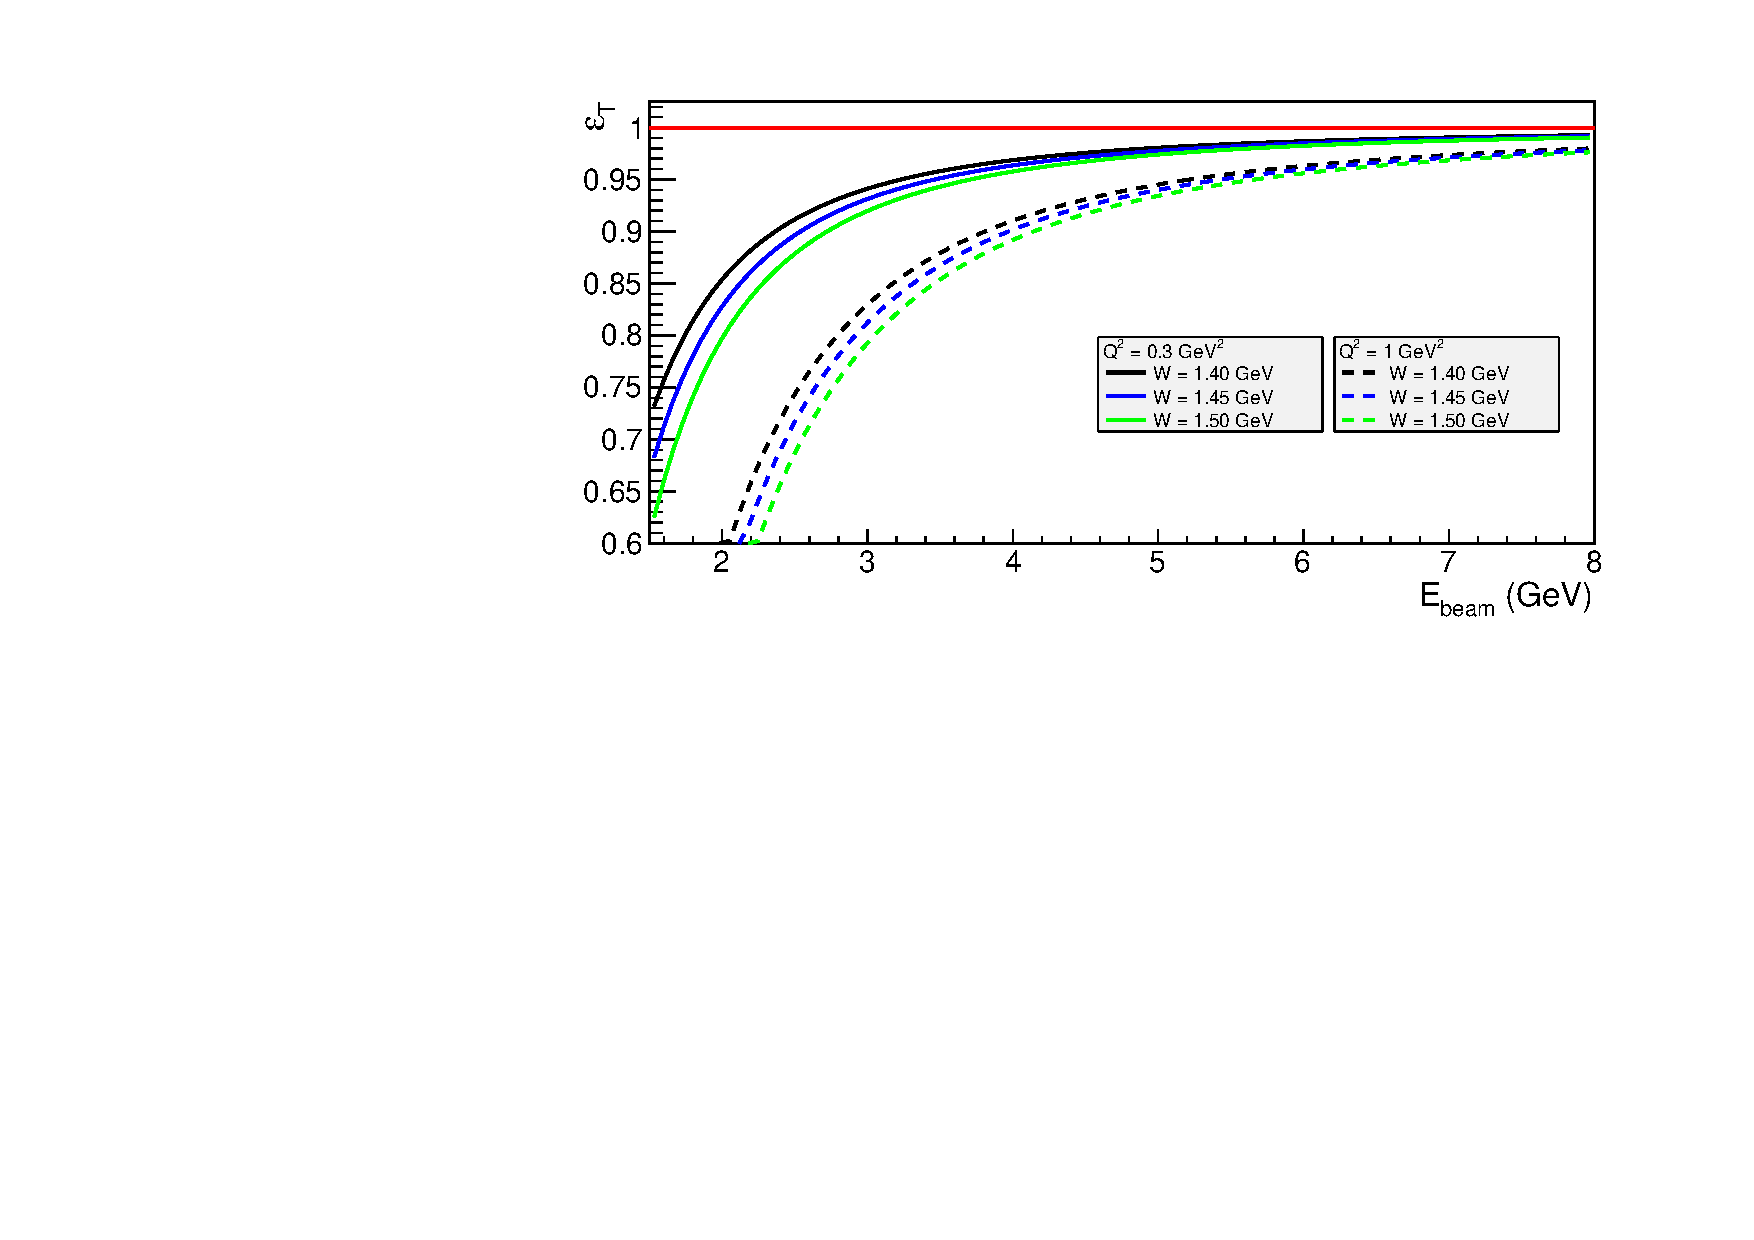
\includegraphics[width=14cm]{pictures/eps_t_dep_ebeam.pdf}}
\end{center}
\caption{\small  The dependence of $\varepsilon_{T}$ on the beam energy given by Eq.~\eqref{eq:dep_on_ebeam} for the case, when the incoming electron moves along the $Z$-axis in the proton rest frame. The upper bunch of the solid curves corresponds to $Q^{2} = 0.3$~GeV$^2$, while the lower bunch of the dashed curves stands for $Q^{2} = 1$~GeV$^2$. Different colors indicate different fixed values of $W$: 1.4~GeV (black), 1.4~GeV (blue), and 1.5~GeV (green). The red line shows the position of unity.}
\label{fig:eps_t_dep_ebeam}
\end{figure}

%\vspace{1cm}

\begin{figure}[!ht]
\begin{center}
\framebox{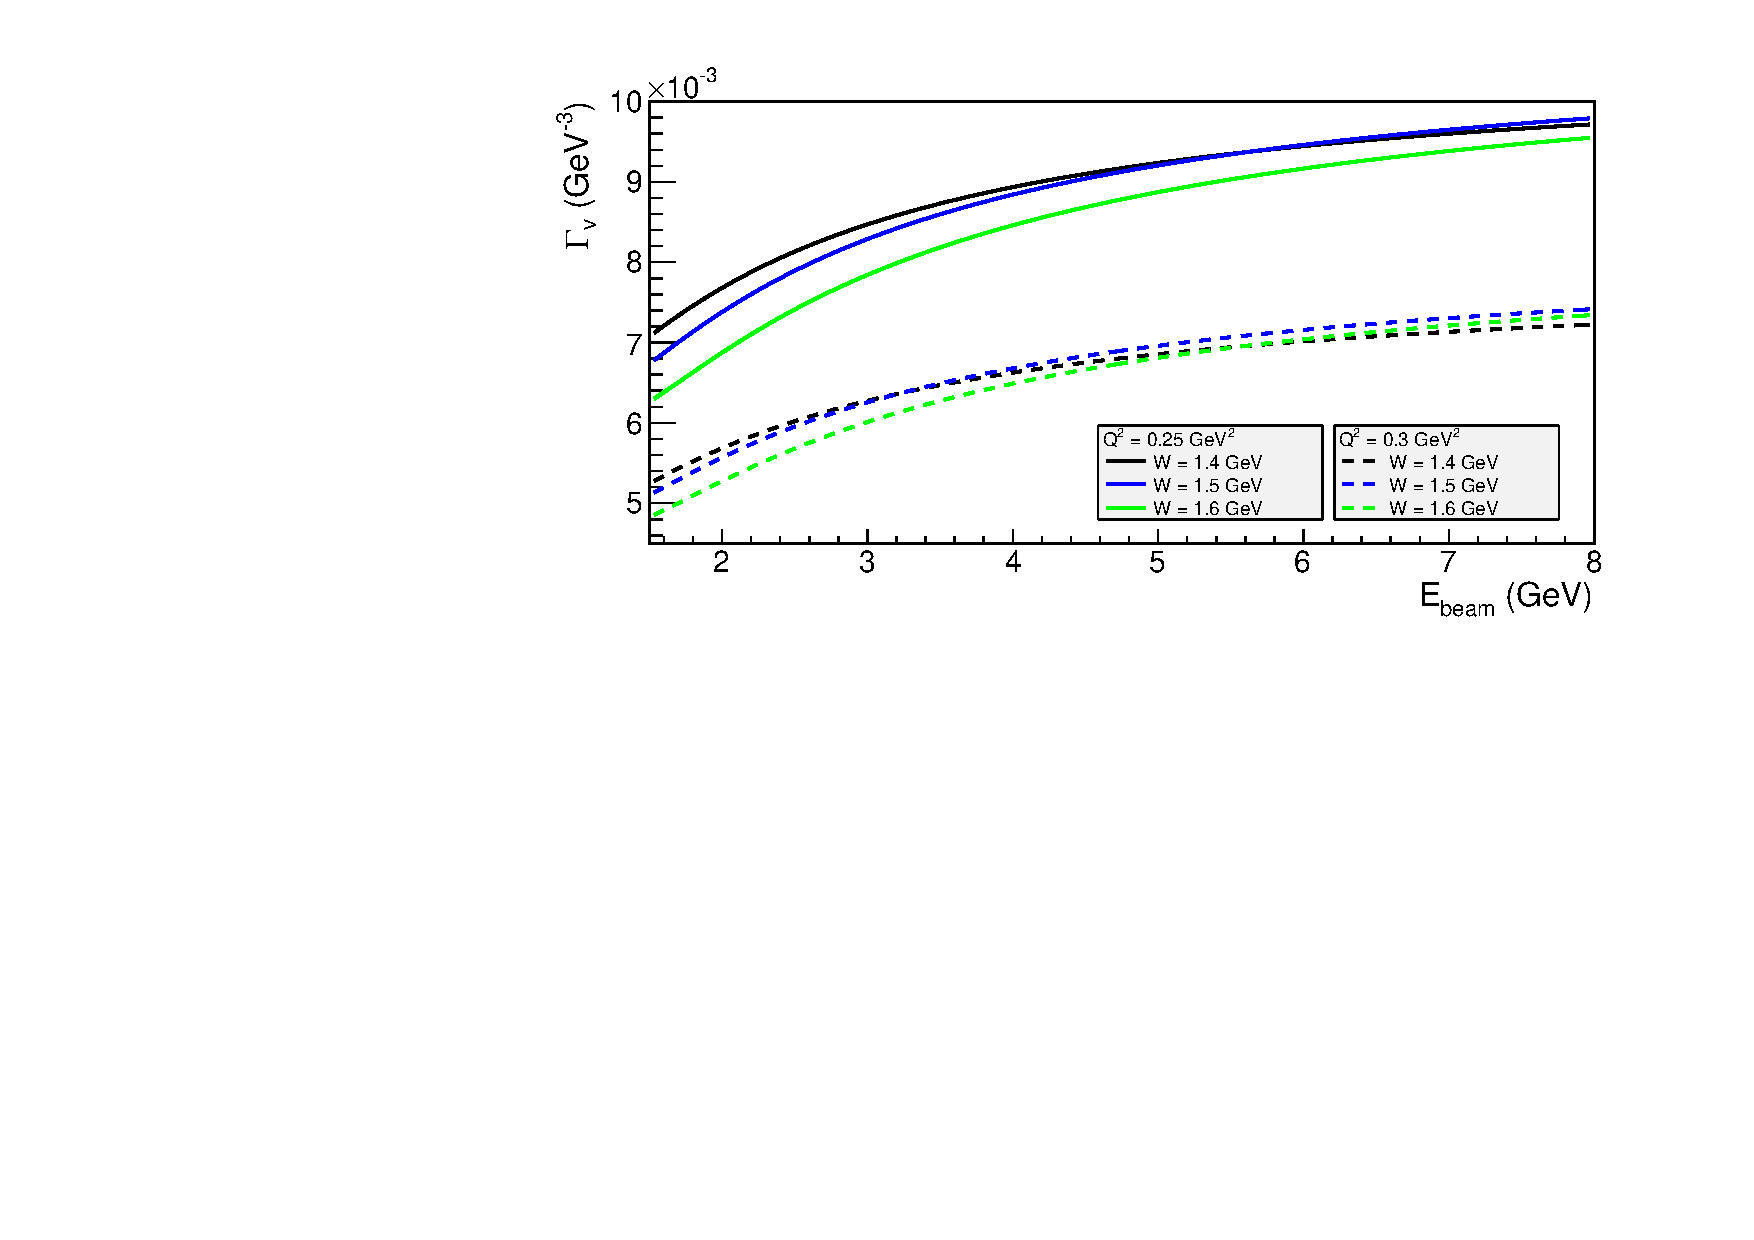
\includegraphics[width=14cm]{pictures/flux_dep_ebeam.pdf}}
\end{center}
\caption{\small  The dependence of $\Gamma_{v}$ on the beam energy for the case, when the incoming electron moves along the $Z$-axis in the proton rest frame. The upper bunch of the solid curves corresponds to $Q^{2} = 0.25$~GeV$^2$, while the lower bunch of the dashed curves stands for $Q^{2} = 0.3$~GeV$^2$. Different colors indicate different fixed values of $W$: 1.4~GeV (black), 1.5~GeV (blue), and 1.6~GeV (green). }
\label{fig:flux_dep_ebeam}
\end{figure}

\clearpage




On top of that, the electroproduction cross section is connected to the virtual photoproduction one via the virtual photon flux $\Gamma_{v}$,  which is also beam energy dependent, as Eq.~(2.2) of the report~\cite{twopeg} demonstrates\footnote[8]{This formula was derived under the assumptions of the incoming electron moving along the Z-axis and the target proton being at rest~\cite{Skorodumina:2016pnb}. }. Figure~\ref{fig:flux_dep_ebeam} illustrates the dependence of the virtual photon flux on the beam energy. The upper bunch of the solid curves again corresponds to the fixed $Q^{2} = 0.25$~GeV$^2$ and the lower bunch of the dashed curves to  $Q^{2} = 0.3$~GeV$^2$. Different colors indicate different fixed values of $W$.



In the proton at rest experiments the conventional practice is to determine $\varepsilon_{T}$, $\varepsilon_{L}$, and $\Gamma_{v}$ in the Lab frame. For the consistency, in the experiments off moving proton these quantities should be defined in the proton rest frame, where the incoming electron has the altered effective beam energy $\widetilde{E}_{beam}$. This circumstance convolutes the extracted cross section with the dependencies of the quantities $\varepsilon_{T}$, $\varepsilon_{L}$, and $\Gamma_{v}$ on the beam energy, hence further complicating the interpretation of the result and its comparison with the cross section of the proton at rest experiment. Although this systematic effect seems not to be significant, it nevertheless should be estimated or corrected for. This can be performed using the proper Monte-Carlo simulation of the reaction under investigation.
 
Section~\ref{sect:proc} describes the calculation of the effective beam energy in TWOPEG-D, while Section~\ref{sect:weights} estimates the influence of the beam energy alteration on the cross section.



%Given by Eq.~\eqref{eps_t} and Eq.~\eqref{eps_l} $\varepsilon_{T}$ and $\varepsilon_{L}$ are invariant under the coordinate axis transformation, but not invariant under the Lorentz boost, while  the expression for $\Gamma_{v}$ (Eq.~(2.2) of the report~\cite{twopeg}) assumes the incoming electron to move along the Z-axis and the target proton to be at rest. 



\section{Blurring of the $Q^{2}$ versus $W$ distribution boundaries}
\label{sect:blur}

In electron scattering experiments the fixed beam energy imposes kinematical limits on the maximal achievable values of $W$ and $Q^2$. 
The kinematical limitations are usually more strongly restricted by the experimental conditions. One of the experimental restrictions comes from the geometrical limitations of the polar angle of the scattered electron. The boundary of the $Q^{2}$ versus $W$ distribution is then determined by

\begin{eqnarray}
Q^2 &=& \frac{2E_{beam}sin^{2}~\frac{\theta_{e'}}{2}\left (2E_{beam}m_{p}-W^{2}+m_{p}^{2}\right )}{m_{p}+2E_{beam}sin^{2}~\frac{\theta_{e'}}{2}},\label{eq:kin_lim}
\end{eqnarray}
where $m_{p}$ is the proton mass and $\theta_{e'}$ is the polar angle of the scattered electron in the Lab frame.

Figure~\ref{fig:kin_lim2} shows the boundary curves determined by Eq.~\eqref{eq:kin_lim} for $E_{beam} = 2$~GeV and three values of $\theta_{e'}$, i.e. $\theta_{e'}^{min}=20^{\circ}$ (dashed blue), $\theta_{e'}^{max}=50^{\circ}$ (dashed magenta), and $\theta_{e'}=180^{\circ}$ (solid black). The last curve stands for the  maximal achievable limit of the $Q^{2}$ versus $W$ distribution.

Beside that, the experimental coverage can be restricted due to the limitation on the minimal detectable energy of the scattered electron $E_{e'}^{min}$. For this case the boundary curve is given by the following relation,

\begin{eqnarray}
Q^2 &=& m_{p}^{2}+2m_{p}(E_{beam} - E_{e'}^{min}) -W^{2}.\label{eq:kin_lim2}
\end{eqnarray}
 
Figure~\ref{fig:kin_lim2} also shows the boundary curve given by Eq.~\eqref{eq:kin_lim2} for the case $E_{e'}^{min}=0.46$~GeV (dotted red).



%These maximal values are connected with each other via Eq.~\eqref{eq:kin_lim}\footnote[8]{The equation is derived from the restriction $|cos~\theta_{e'}|<1$, where $cos~\theta_{e'} = 1-\frac{Q^2}{2E_{beam}E_{e'}}$.}, which determines the envelope of the experimental $Q^{2}$ versus $W$ distribution.
%These maximal values belong to the curve given by Eq.~\eqref{eq:kin_lim}\footnote[8]{The equation is derived from the restriction $|cos~\theta_{e'}|<1$, where $cos~\theta_{e'} = 1-\frac{Q^2}{2E_{beam}E_{e'}}$}.


\begin{figure}[!ht]
\begin{center}
\framebox{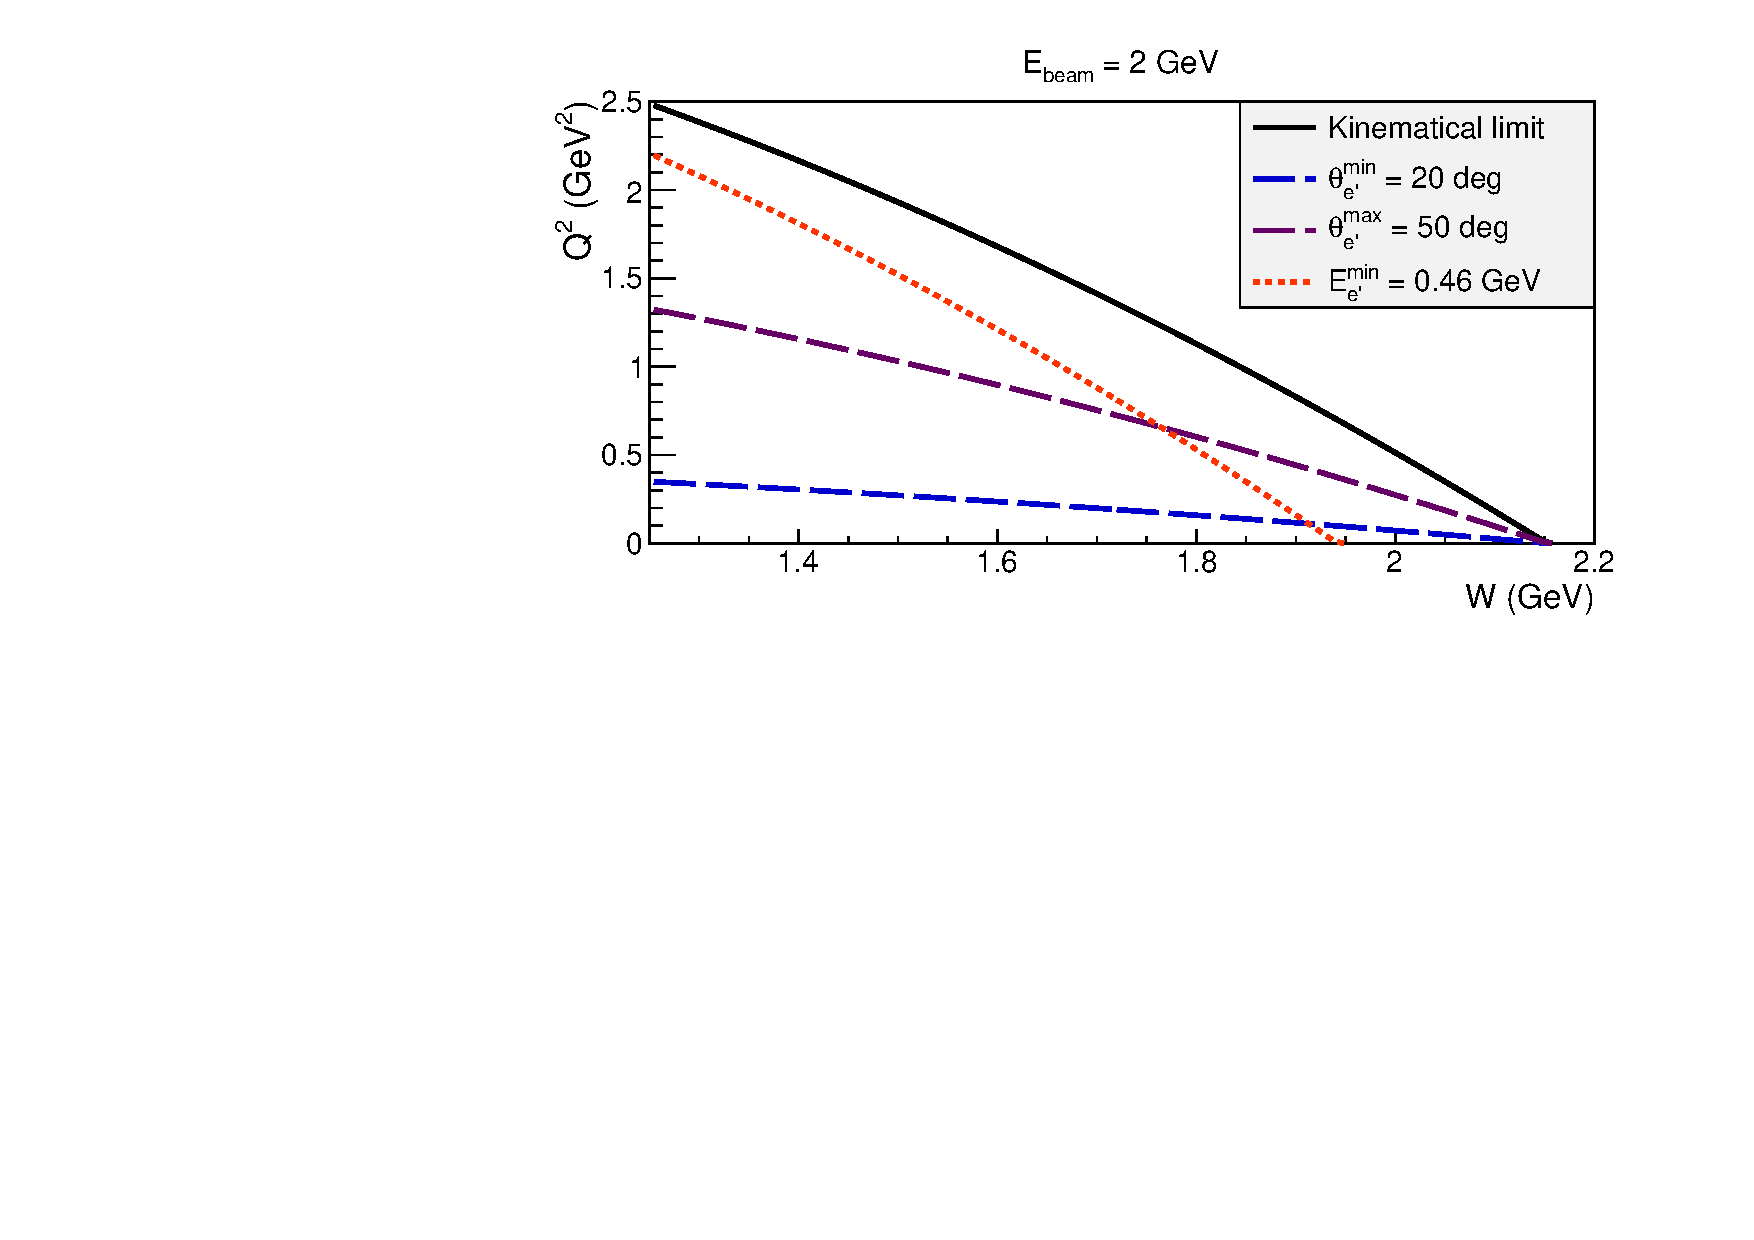
\includegraphics[width=14cm]{pictures/kin_lim2.pdf}}
\end{center}
\caption{\small  The margins of the $Q^{2}$ versus $W$ distribution for an experiment conducted with 2 GeV beam energy. The solid black curve shows the maximal achievable boundary and is given by Eq.~\eqref{eq:kin_lim} with $\theta_{e'}=180^{\circ}$. The dashed blue and magenta curves stand for the edges due to the limitation of the polar angle of the scattered electron. They are given by Eq.~\eqref{eq:kin_lim} for $\theta_{e'}^{min}=20^{\circ}$ and $\theta_{e'}^{max}=50^{\circ}$, respectively. The dotted red curve shows the edge due to the limitation on the minimal detectable energy of the scattered electron and is given by Eq.~\eqref{eq:kin_lim2} for $E_{e'}^{min} = 0.46$~GeV.}
\label{fig:kin_lim2}
\end{figure}

The edges of the $Q^{2}$ versus $W$ distribution given by Eqs.~\eqref{eq:kin_lim} and~\eqref{eq:kin_lim2} are beam energy dependent. As written above, the experiment off the moving proton with fixed beam energy is equivalent to that off the proton at rest performed with altered effective beam energy. Therefore, the distribution edges, being sharp and distinct in the proton at rest experiment, become blurred in the experiment off the moving proton.

Let's consider a moving proton experiment conducted with 2 GeV beam energy and assume the deviation of the effective beam energy from this value to be $\pm 250$~MeV. This situation is illustrated in Fig.~\ref{fig:kin_lim}, where the maximal achievable boundaries are shown for three choices of the beam energy: 2 GeV (solid black curve), 1.75 GeV (dashed blue curve), and 2.25 GeV (dashed magenta curve). The region between the two dashed curves shows the scope of the expected blurring. 
The boundaries caused by the experimental restrictions (the dashed and dotted curves in Fig.~\ref{fig:kin_lim2}), being also beam energy dependent, are subject to the analogous blurring.
%Other boundaries given by Eq.~\eqref{eq:kin_lim} and Eq.~\eqref{eq:kin_lim2}, being also beam energy dependent, are subject to the analogous blurring.


\begin{figure}[!ht]
\begin{center}
\framebox{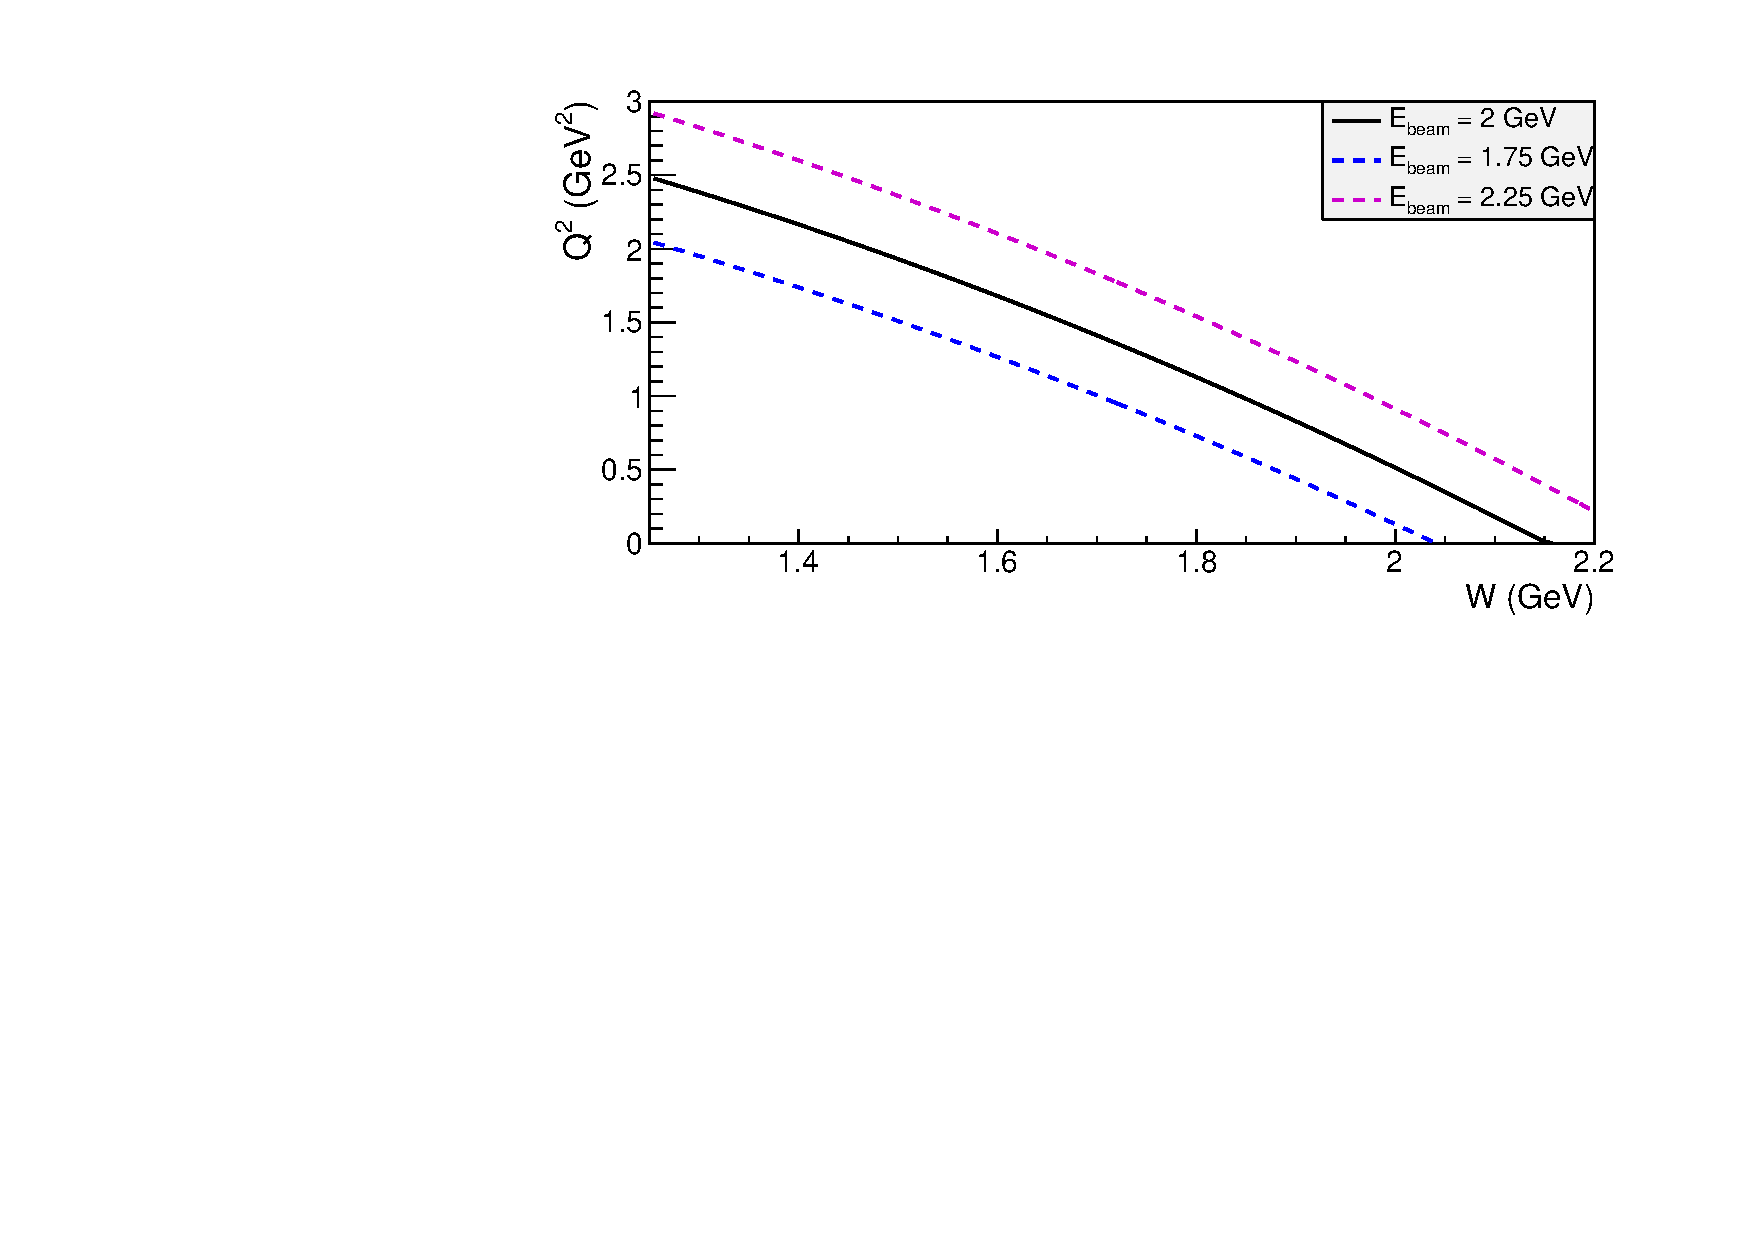
\includegraphics[width=14cm]{pictures/kin_lim.pdf}}
\end{center}
\caption{\small  The illustration of blurring of the maximal achievable limit of the $Q^{2}$ versus $W$ distribution. The curves are given by Eq.~\eqref{eq:kin_lim} for the case $\theta_{e'}=180^{\circ}$ and three choices of beam energy. }
\label{fig:kin_lim}
\end{figure}


The event yield in the blurring region suffers from the depletion of events (compared to that for the case of fixed beam energy and sharp disrtribution edge). To estimate this effect, one should know the function that describes the alteration of the effective beam energy. This function is in turn determined by the target proton momentum distribution.
The cross sections extracted in the blurring region need a special correction, otherwise they will suffer from underestimation. This correction requires  either experimental knowledge on initial proton momentum for each reaction event or  the proper Monte Carlo simulation of the blurring effect. 


Note that Eqs.~\eqref{eq:kin_lim} and~\eqref{eq:kin_lim2} as well as Figs.~\ref{fig:kin_lim2} and~\ref{fig:kin_lim} assume the value of $W$ to be the true value of the invariant mass of the final hadron system given by Eq.~\eqref{W_fin_2}. Only in this case the boundary blurring takes place. If the smeared value of $W$, calculated under the target-at-rest assumption, is used instead, the distribution edges are not subject to this blurring because the fixed value of the laboratory beam energy is used in calculations.


 




